\chapter{Advanced Protection Schemes} \label{ch_5}
\section{Introduction}
Limitations of existing Protection technology.The existing protection and control applications have been working for many years assuming the conventional grid architecture, and they have performed exceptionally well thus far. However, modern power systems dynamics have changed, leading to protection and control facing new challenges to maintain/improve the network and asset performance  metrics.\\
Opportunities for AI in Protection.\\
Increasing availability of large amounts of high-fidelity, rapidly sampled data, both in time domain and frequency domain is enabling the development and deployment of AI/ML-based solutions to challenging protection and control problems. \\
Some drivers leading the focus towards the Artificial Intelligence are: \\
● High penetration of Distributed Energy Resources , Large scale inverter-based resources \\
● Growing need for advanced distribution protection and control applications including fault detection and location \\
● Power system reconfiguration \\
Need for improving the efficiency in protection systems design and engineering 
There are many existing applications and emerging applications in literature.\\

Existing Applications \\
		AI to Detect Secondary Arc \\
		Hybrid Intelligent Model for Protection Settings Optimization
 	Emerging Applications \\
		High-Impedance Fault Detection with ANN. \\
		Synchrophasor and ML for Early Detection of Voltage Instability\\
		Detecting Relay Misoperations Using Field Data \\ 
		Application of AI/ML in Travelling Wave Protection\\
			TW Protection of AC Distribution Systems Using ML \\
			 TW Protection of DC Systems Using ML \\





\section{AI to Enhance Protection in Active DNs}

Improve Distribution System Operational Parameters Utilizing Smart Inverter Functionalities of PV Sources.\\

First, we scenario of using Intelligent method utilizing smart inverter functionalities of a PV source in a distribution network is proposed in present work to minimize, the power import from the grid, reduce network losses and minimize the magnitude of voltage violation. The optimal settings depend on  load and generation variables. In order to reduce computational complexity, a scenario-based method is used to handle these stochastic components in the system. A Non-Sorted Genetic Algorithm (NSGA) is used for optimizing the smart inverters parameters. The proposed scheme is envisaged to be realized by a Distribution Management System (DMS) which measures and coordinates all the smart inverters within the distribution feeder.\\

\begin{figure}[!ht]
	\centering
    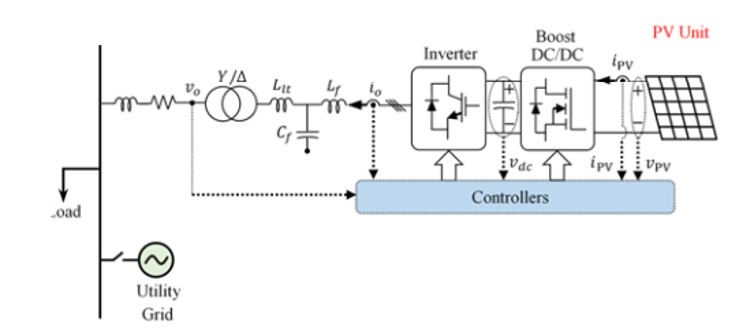
\includegraphics[width=0.95\columnwidth]{images/chapter_5/Ch5F1.jpg}
	\caption{Control of Smart Inverter}
	\label{fig_MG}
\end{figure}

\begin{figure}[!ht]
	\centering
    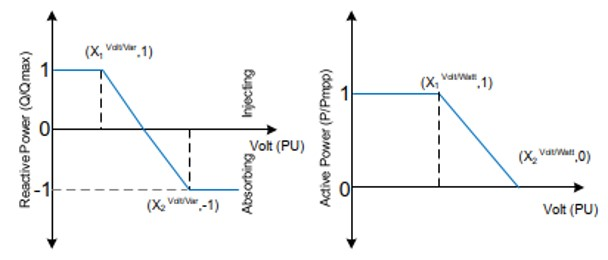
\includegraphics[width=0.95\columnwidth]{images/chapter_5/Ch5F2.jpg}
	\caption{Volt-Var and Volt-Watt control characteristics of 
the Smart Inverter.}
	\label{fig_MG}
\end{figure}


\begin{figure}[!ht]
	\centering
    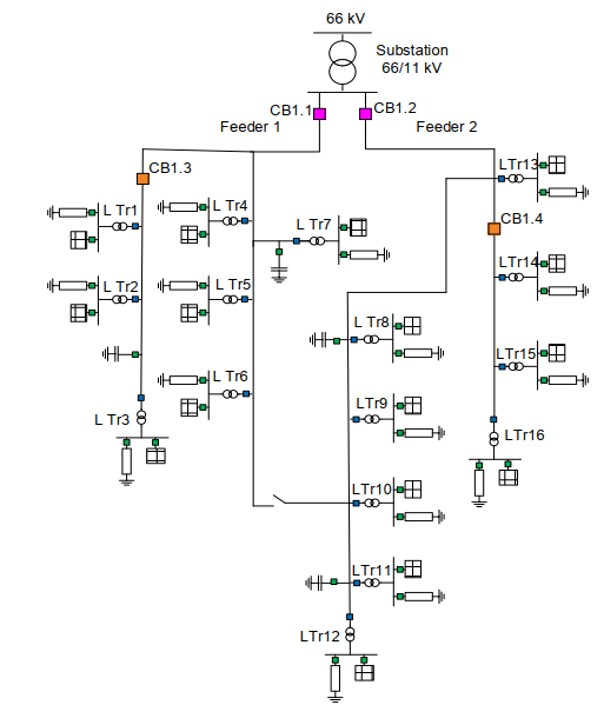
\includegraphics[width=0.95\columnwidth]{images/chapter_5/Ch5F3.jpg}
	\caption{Case study network.}
	\label{fig_MG}
\end{figure}

\begin{figure}[!ht]
	\centering
    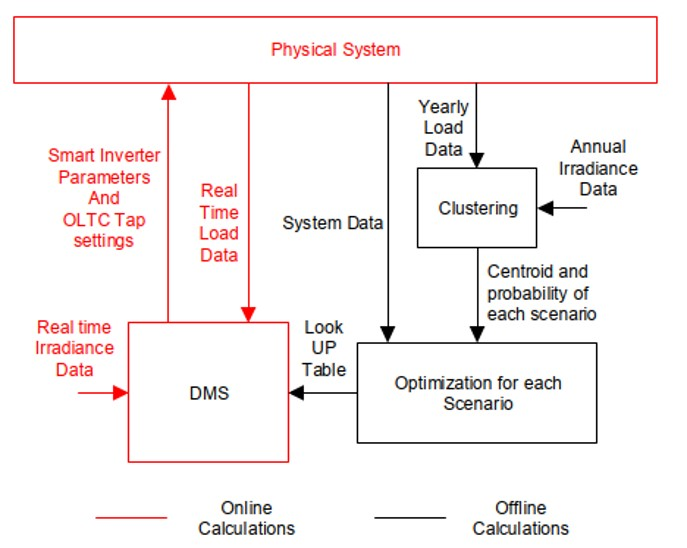
\includegraphics[width=0.95\columnwidth]{images/chapter_5/Ch5F4.jpg}
	\caption{Information flow diagram for proposed method .}
	\label{fig_MG}
\end{figure}

\begin{figure}[!ht]
	\centering
    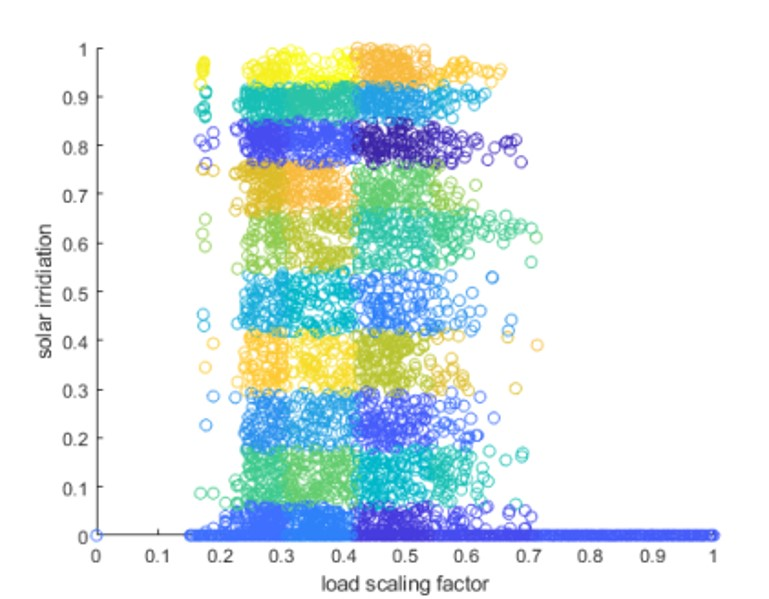
\includegraphics[width=0.95\columnwidth]{images/chapter_5/Ch5F5.jpg}
	\caption{Final clustering data.}
	\label{fig_MG}
\end{figure}

\begin{figure}[!ht]
	\centering
    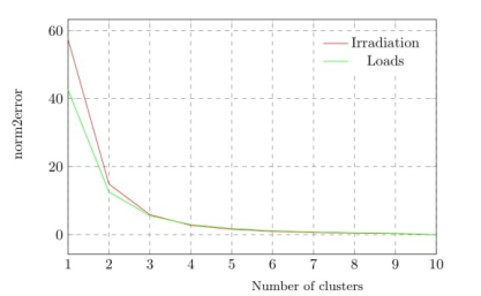
\includegraphics[width=0.95\columnwidth]{images/chapter_5/Ch5F6.jpg}
	\caption{norm2error Vs number of clusters.}
	\label{fig_MG}
\end{figure}

\begin{figure}[!ht]
	\centering
    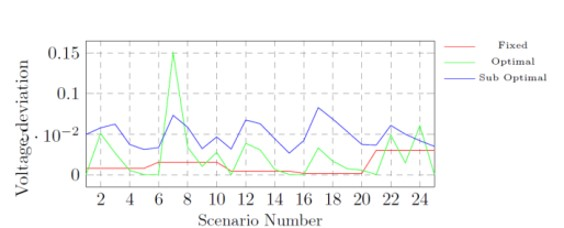
\includegraphics[width=0.95\columnwidth]{images/chapter_5/Ch5F7.jpg}
	\caption{Voltage variation for each scenario.}
	\label{fig_MG}
\end{figure}

\begin{figure}[!ht]
	\centering
    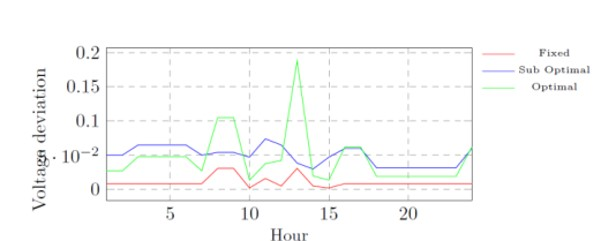
\includegraphics[width=0.95\columnwidth]{images/chapter_5/Ch5F8.jpg}
	\caption{Voltage variations for typical daily data.}
	\label{fig_MG}
\end{figure}


\begin{figure}[!ht]
	\centering
    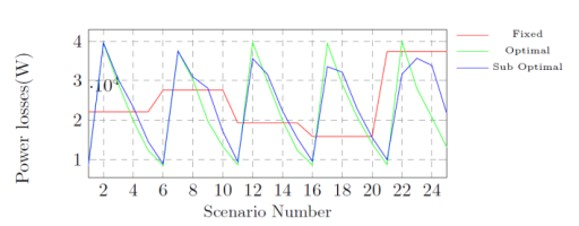
\includegraphics[width=0.95\columnwidth]{images/chapter_5/Ch5F9.jpg}
	\caption{Power losses for each scenario.}
	\label{fig_MG}
\end{figure}

\begin{figure}[!ht]
	\centering
    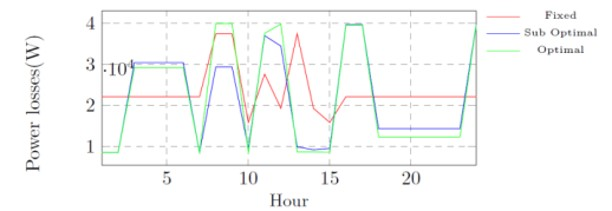
\includegraphics[width=0.95\columnwidth]{images/chapter_5/Ch5F10.jpg}
	\caption{Loss variations for typical daily data.}
	\label{fig_MG}
\end{figure}

\begin{figure}[!ht]
	\centering
    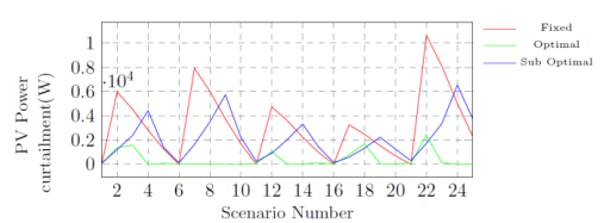
\includegraphics[width=0.95\columnwidth]{images/chapter_5/Ch5F11.jpg}
	\caption{PV power curtailment for each scenario.}
	\label{fig_MG}
\end{figure}

\begin{figure}[!ht]
	\centering
    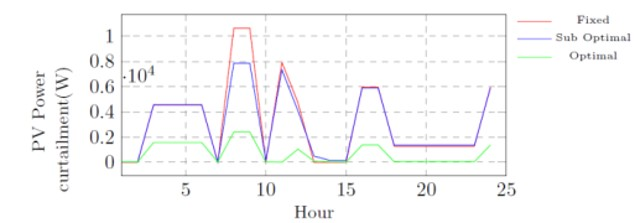
\includegraphics[width=0.95\columnwidth]{images/chapter_5/Ch5F12.jpg}
	\caption{PV curtailment  for typical daily data.}
	\label{fig_MG}
\end{figure}

\section{Transform-Domain Deep Convolutional Network for Fault Detection and Classification}
In network with high penetration of PV sources SPM of fault voltages incudes transients and noises. Curve fitting based estimation of SPM parameters cause error.\\
We use CNN to classify events and estimate fault category.
Convolutional neural networks (CNNs) are one type of deep learning methods developed specifically to learn the hierarchical representation of input data, as well as to predict the class label of the data. \\

Fault detection and classification using deep convolutional neural networks.\\
Employ the deep learning in an effective three-dimensional (3-D) transform domain, under space-phasor model (SPM), for efficient learning of Events.\\
Characterize fault voltage dips by 2-D SPM-based deep learning, which leads to fault classification independent of the duration and sampling frequency.\\

\begin{figure}[!ht]
	\centering
    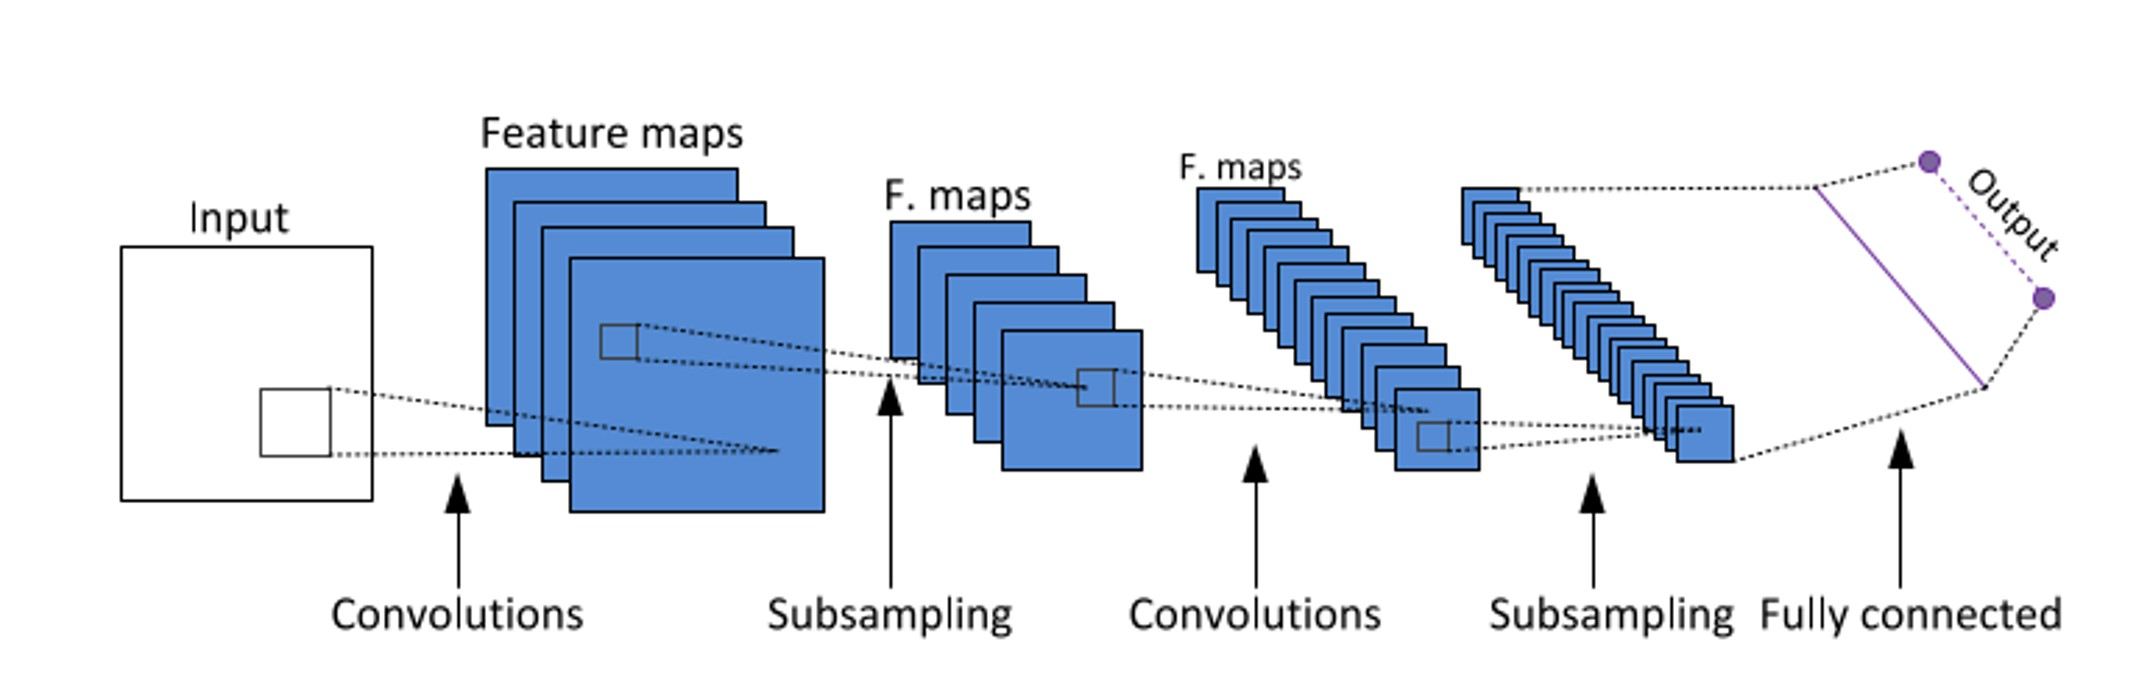
\includegraphics[width=0.95\columnwidth]{images/chapter_5/Ch5F13.jpg}
	\caption{Figure Typical architecture of a Convolutional Neural Networks}
\end{figure}
    
\begin{table}[h]
    \centering
    \begin{tabular}{|l|c|c|}
    \hline
    \textbf{Layer (type)} & \textbf{Output Shape} & \textbf{Param \#} \\
    \hline
    input\_1 (InputLayer) & [(None, 8, 8, 6, 1)] & 0 \\
    \hline
    conv3d (Conv3D) & (None, 7, 7, 5, 64) & 576 \\
    \hline
    max\_pooling3d (MaxPooling3D) & (None, 7, 7, 5, 64) & 0 \\
    \hline
    batch\_normalization (BatchNormalization) & (None, 7, 7, 5, 64) & 256 \\
    \hline
    conv3d\_1 (Conv3D) & (None, 6, 6, 4, 64) & 32832 \\
    \hline
    max\_pooling3d\_1 (MaxPooling3D) & (None, 6, 6, 4, 64) & 0 \\
    \hline
    batch\_normalization\_1 (BatchNormalization) & (None, 6, 6, 4, 64) & 256 \\
    \hline
    conv3d\_2 (Conv3D) & (None, 4, 4, 3, 128) & 8320 \\
    \hline
    max\_pooling3d\_2 (MaxPooling3D) & (None, 3, 3, 2, 128) & 0 \\
    \hline
    batch\_normalization\_2 (BatchNormalization) & (None, 3, 3, 2, 128) & 512 \\
    \hline
    global\_average\_pooling3d (GlobalAveragePooling3D) & (None, 128) & 0 \\
    \hline
    dense (Dense) & (None, 512) & 66048 \\
    \hline
    dropout (Dropout) & (None, 512) & 0 \\
    \hline
    dense\_1 (Dense) & (None, 4) & 2052 \\
    \hline
    \end{tabular}
    \caption{3dCNN Model Layers}
    \label{tab:3dcnn_model}
\end{table}
	\label{fig_MG}


In a CNN, the input data is first transformed through a series of chained convolutional filters with nonlinear activation functions which is equivalent to applying a series of chained multichannel nonlinear filters. By stacking multiple convolution layers with nonlinear activation functions in between, it allows the network to learn sophisticated features of the data. The network is then followed by a series of fully connected (FC) layers with nonlinear activation functions in between. This results in an output vector of class probabilities after the softmax activation function in the last FC layer. Both parts of the network are usually trained together for obtaining the best network architecture, filter coefficients/weights by adjusting the number of layers, the number of filters and their size and hyper-parameters, such that satisfactory end-to-end performance is obtained under a selected objective criterion or loss function.


\begin{figure}[!ht]
	\centering
    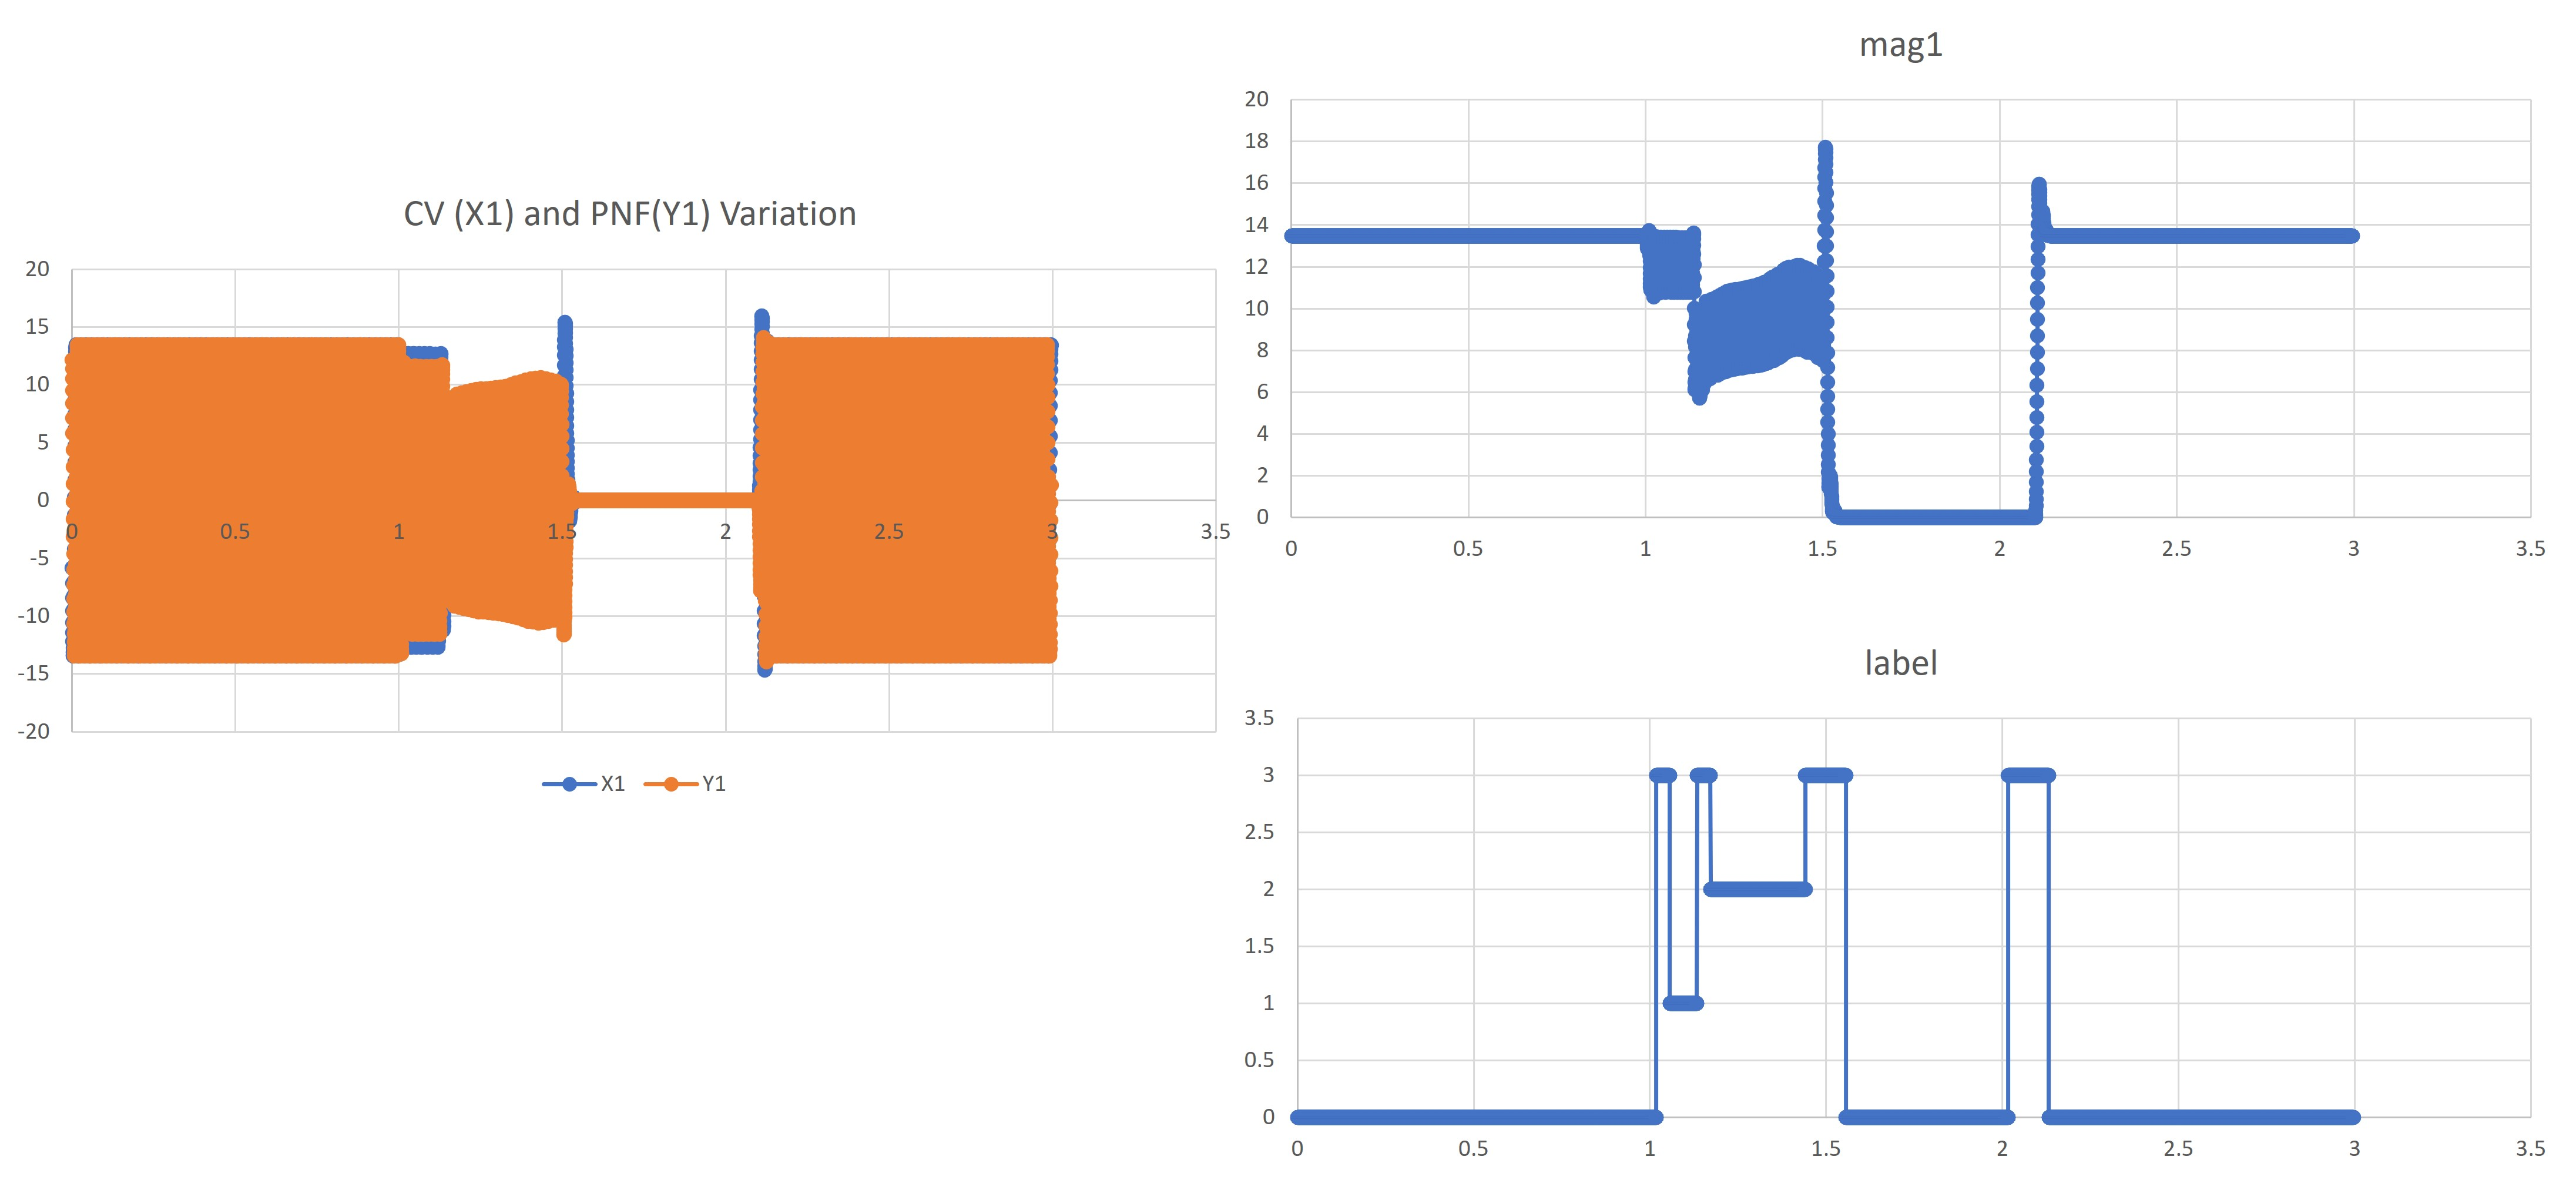
\includegraphics[width=0.95\columnwidth]{images/chapter_5/Ch5F14.jpg}
	\caption{Figure Typical architecture of a Convolutional Neural Networks}
\end{figure}

\begin{figure}[!ht]
	\centering
    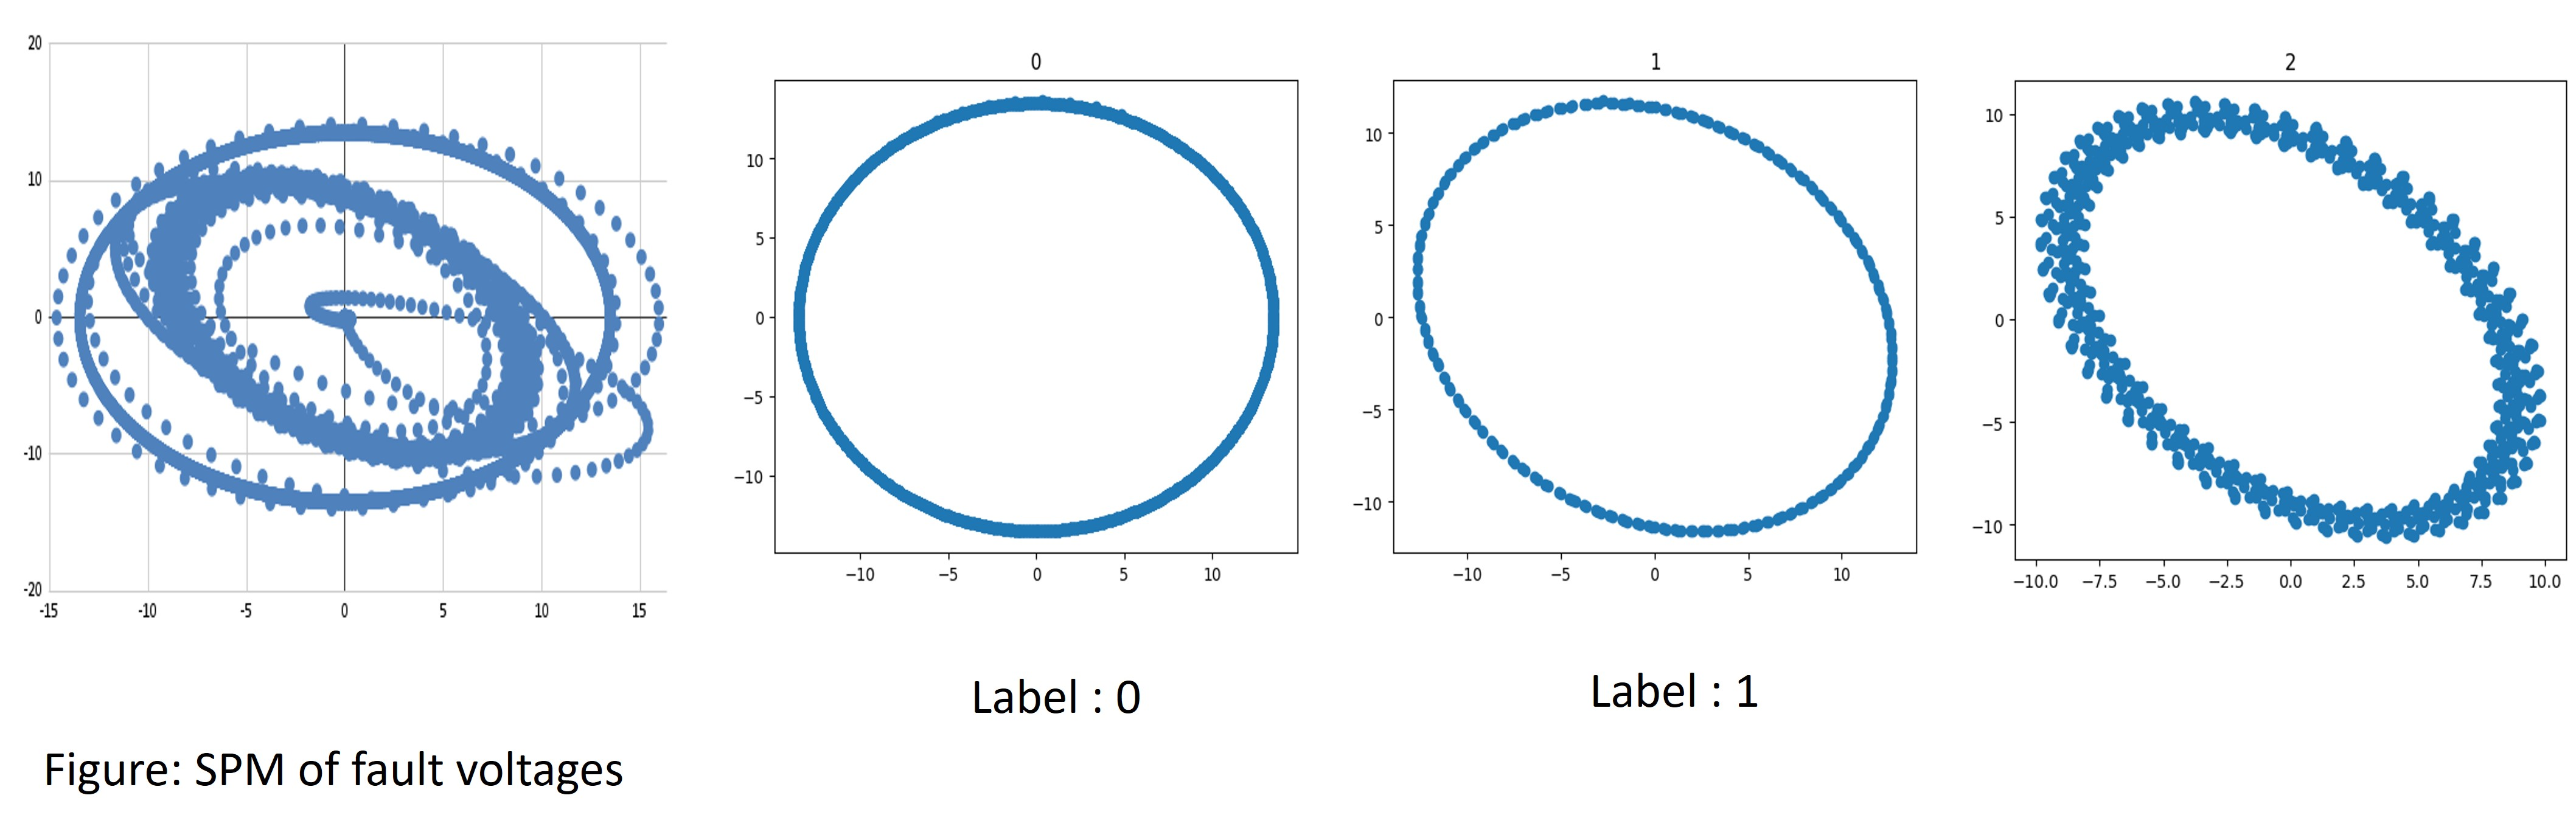
\includegraphics[width=0.95\columnwidth]{images/chapter_5/Ch5F15.jpg}
	\caption{Figure Typical architecture of a Convolutional Neural Networks}
\end{figure}

\begin{figure}[!ht]
	\centering
    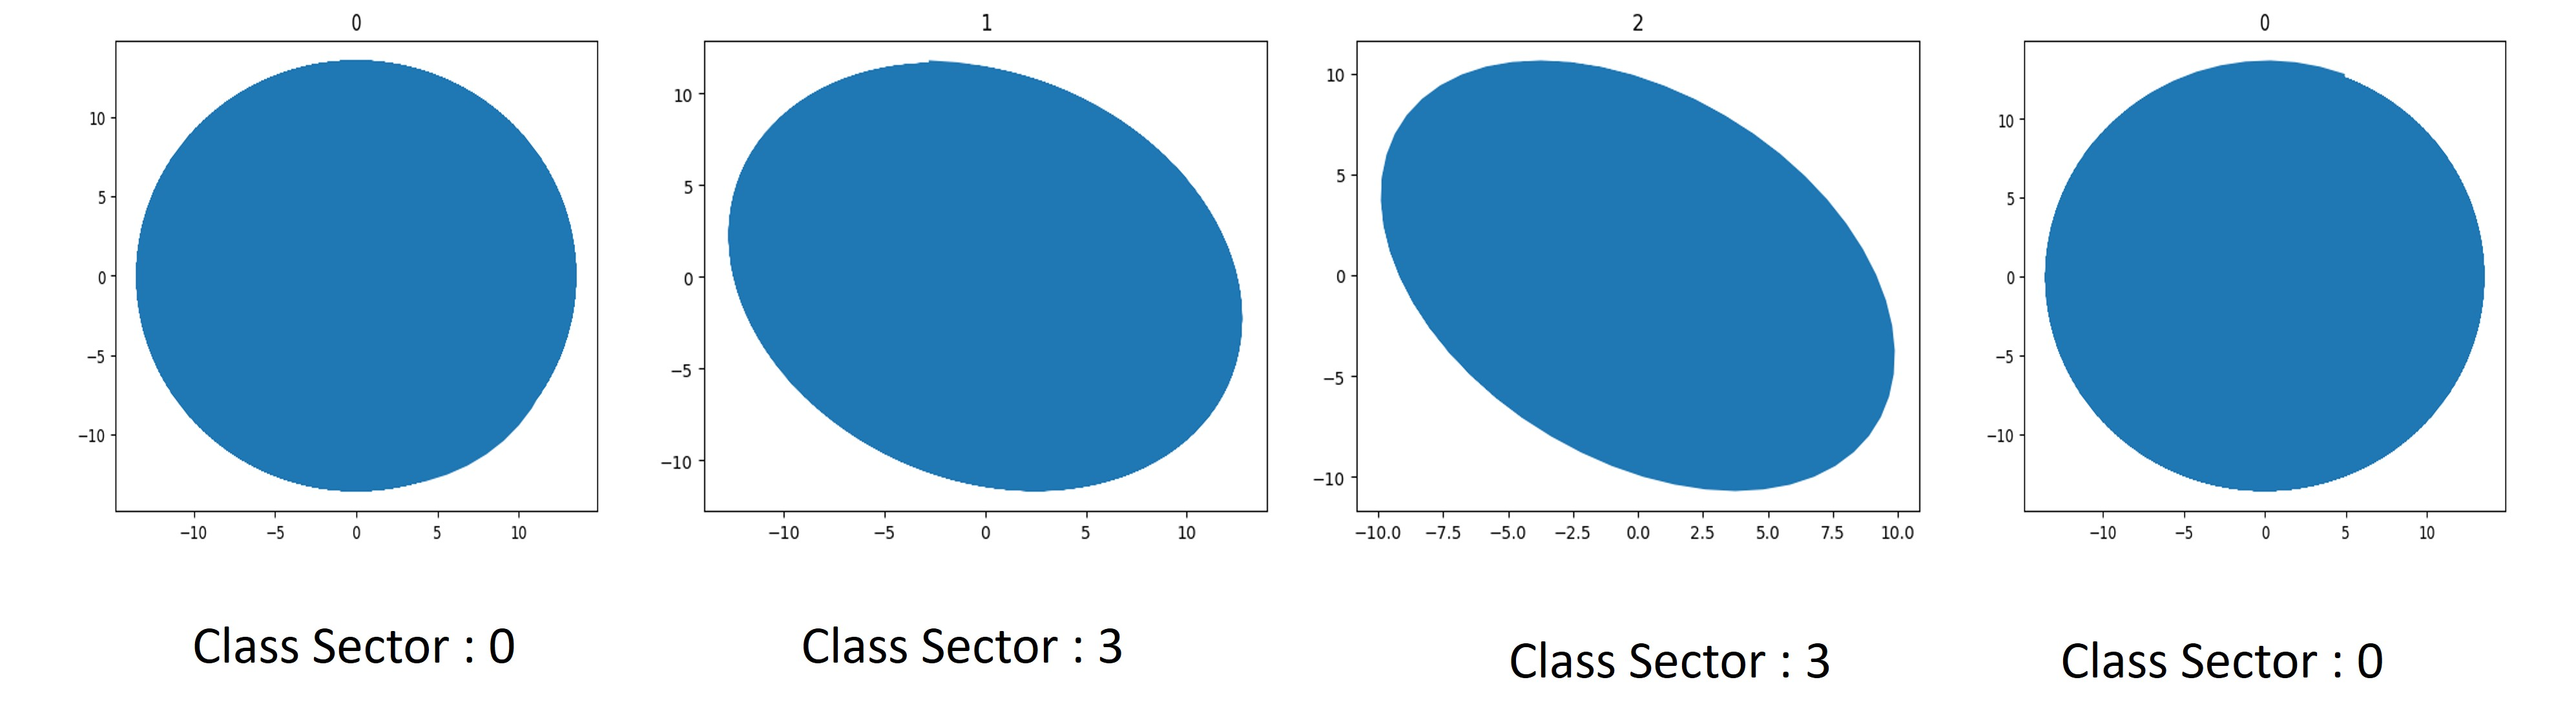
\includegraphics[width=0.95\columnwidth]{images/chapter_5/Ch5F16.jpg}
	\caption{Figure Typical architecture of a Convolutional Neural Networks}
\end{figure}

\begin{figure}[!ht]
	\centering
    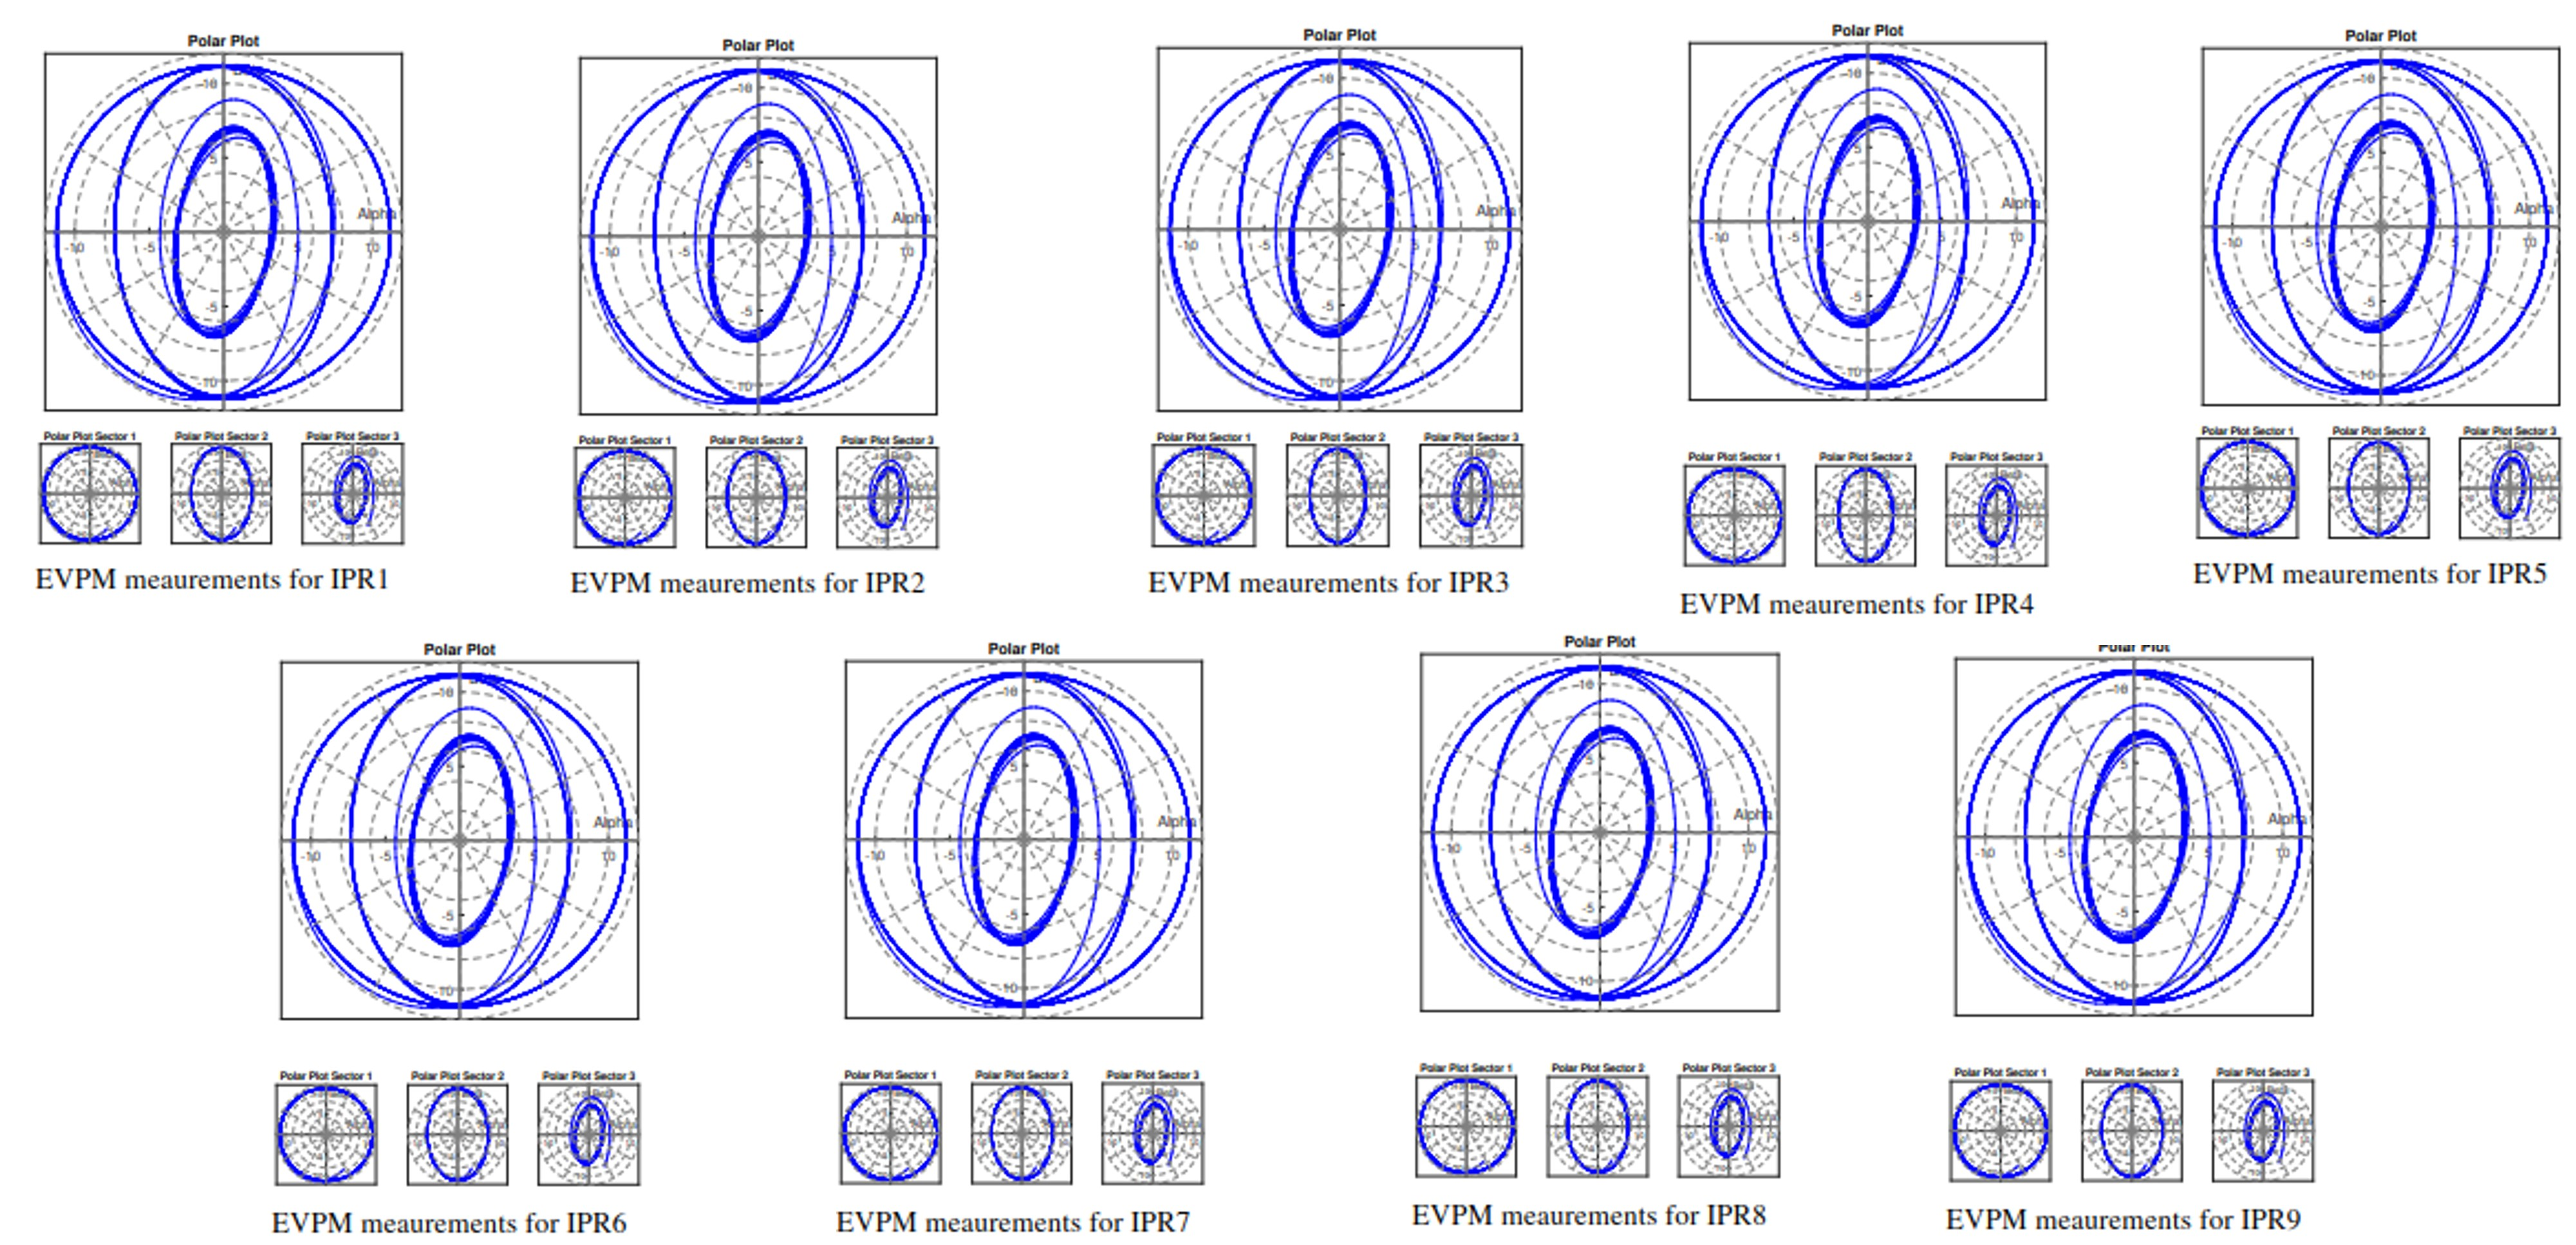
\includegraphics[width=0.95\columnwidth]{images/chapter_5/Ch5F17.jpg}
	\caption{Figure Typical architecture of a Convolutional Neural Networks}
\end{figure}

\begin{figure}[!ht]
	\centering
    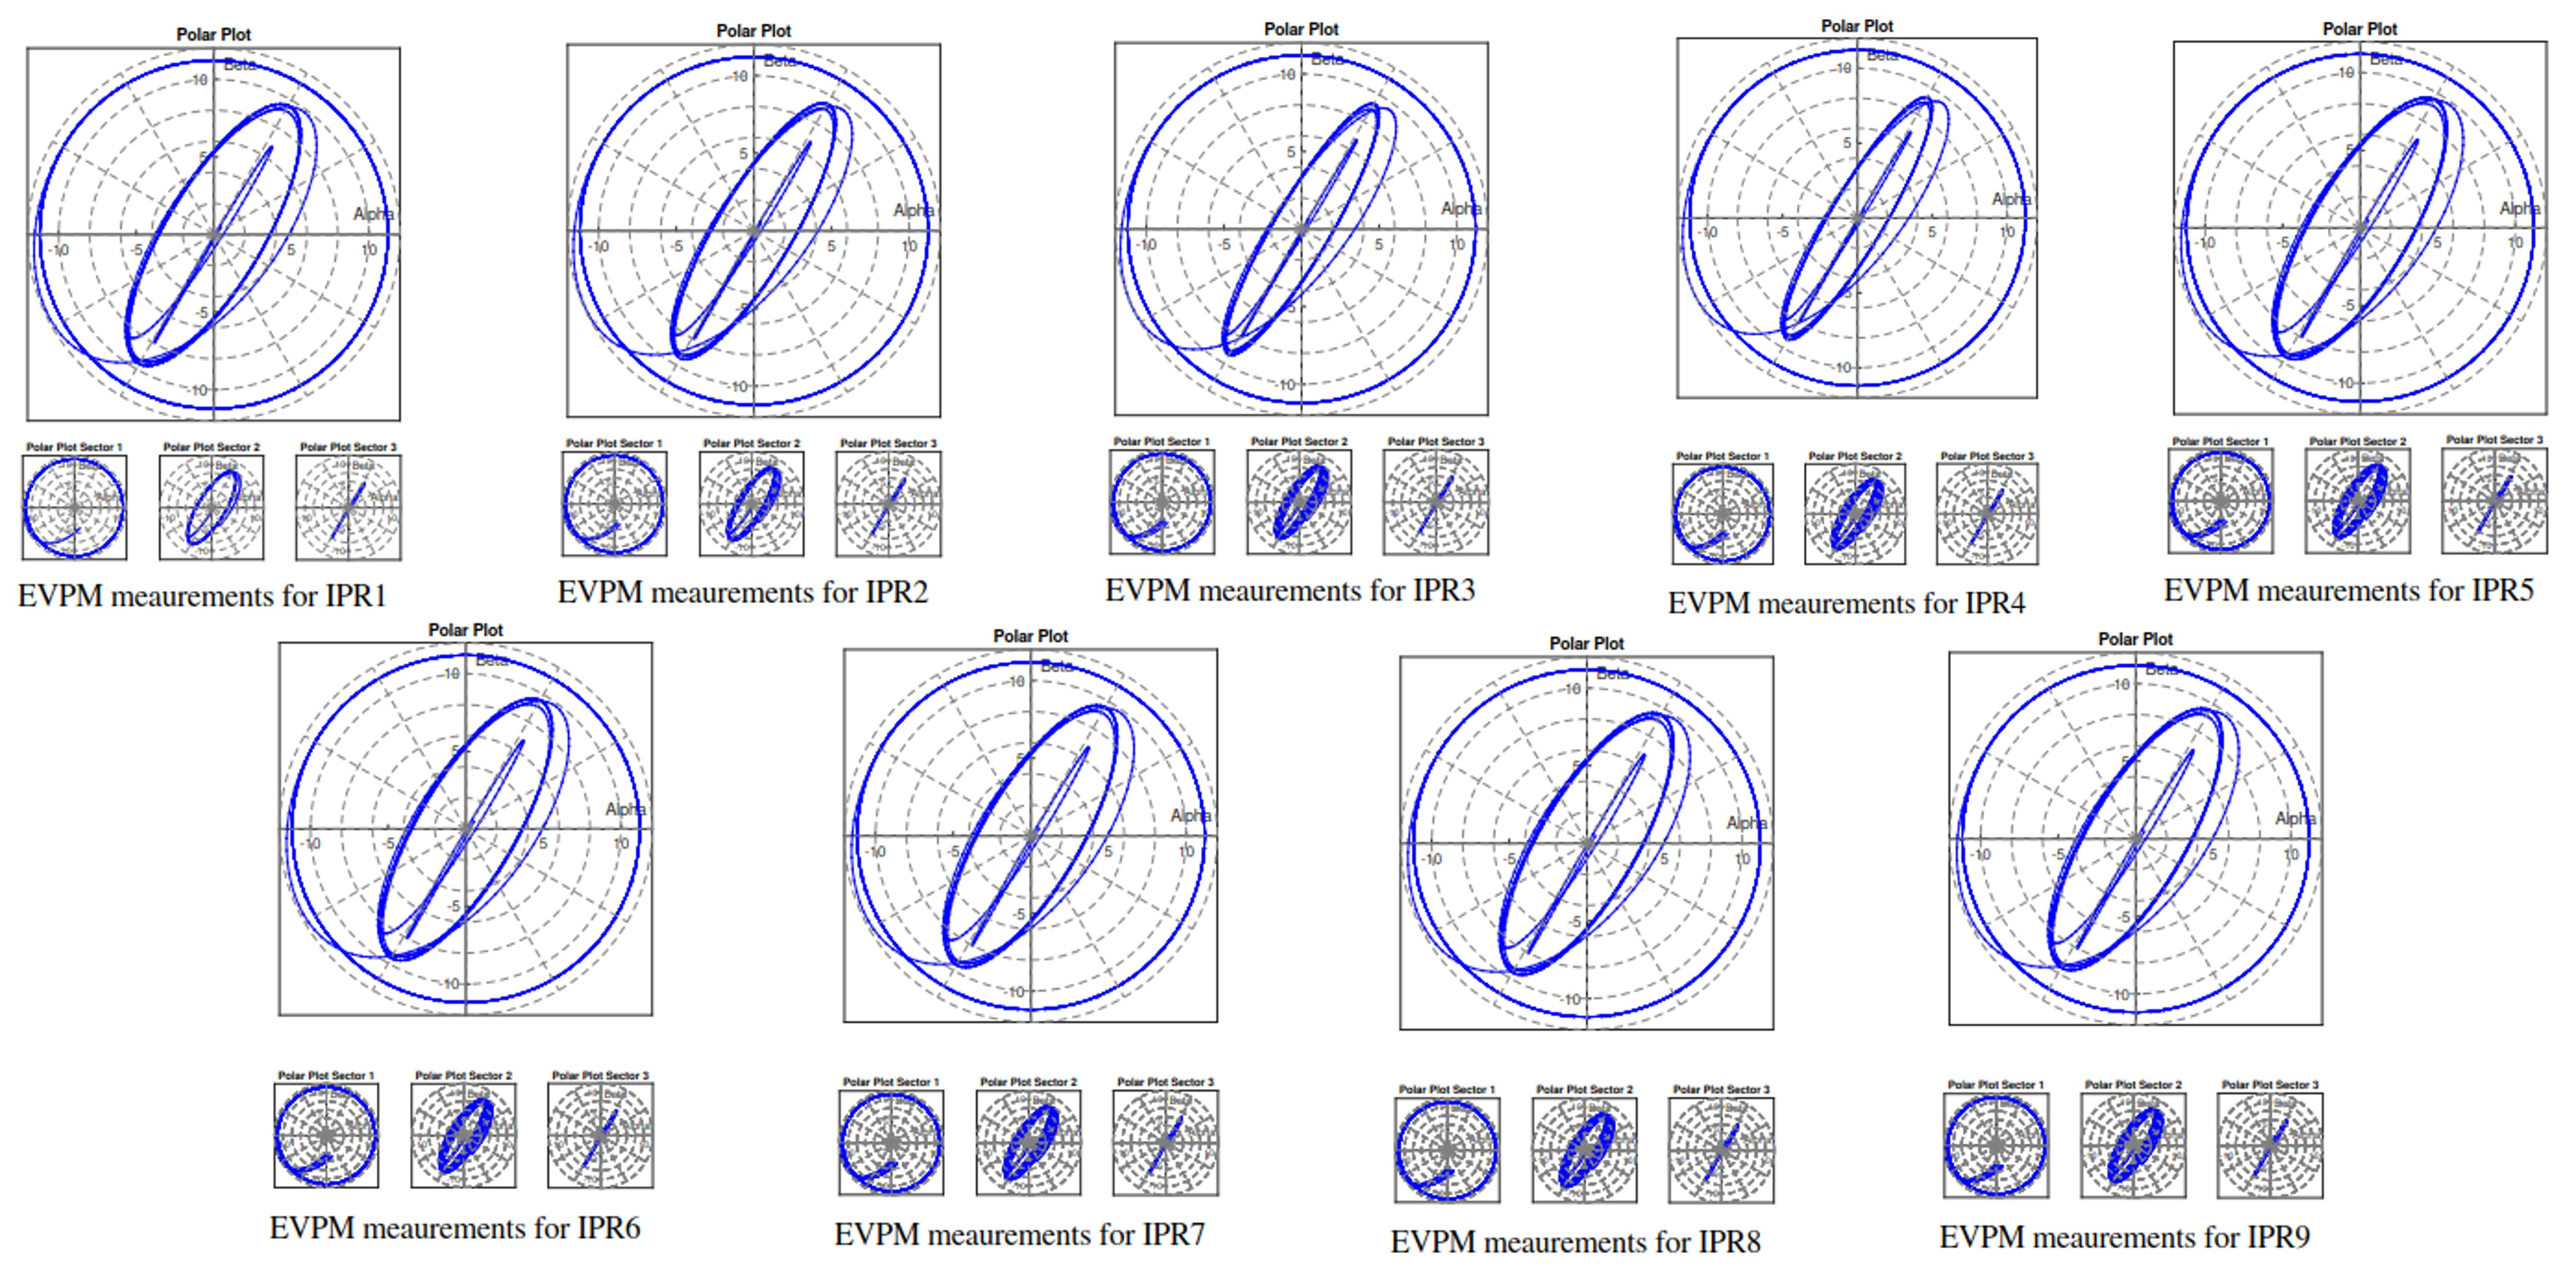
\includegraphics[width=0.95\columnwidth]{images/chapter_5/Ch5F18.jpg}
	\caption{Figure Typical architecture of a Convolutional Neural Networks}
\end{figure}

\begin{figure}[!ht]
	\centering
    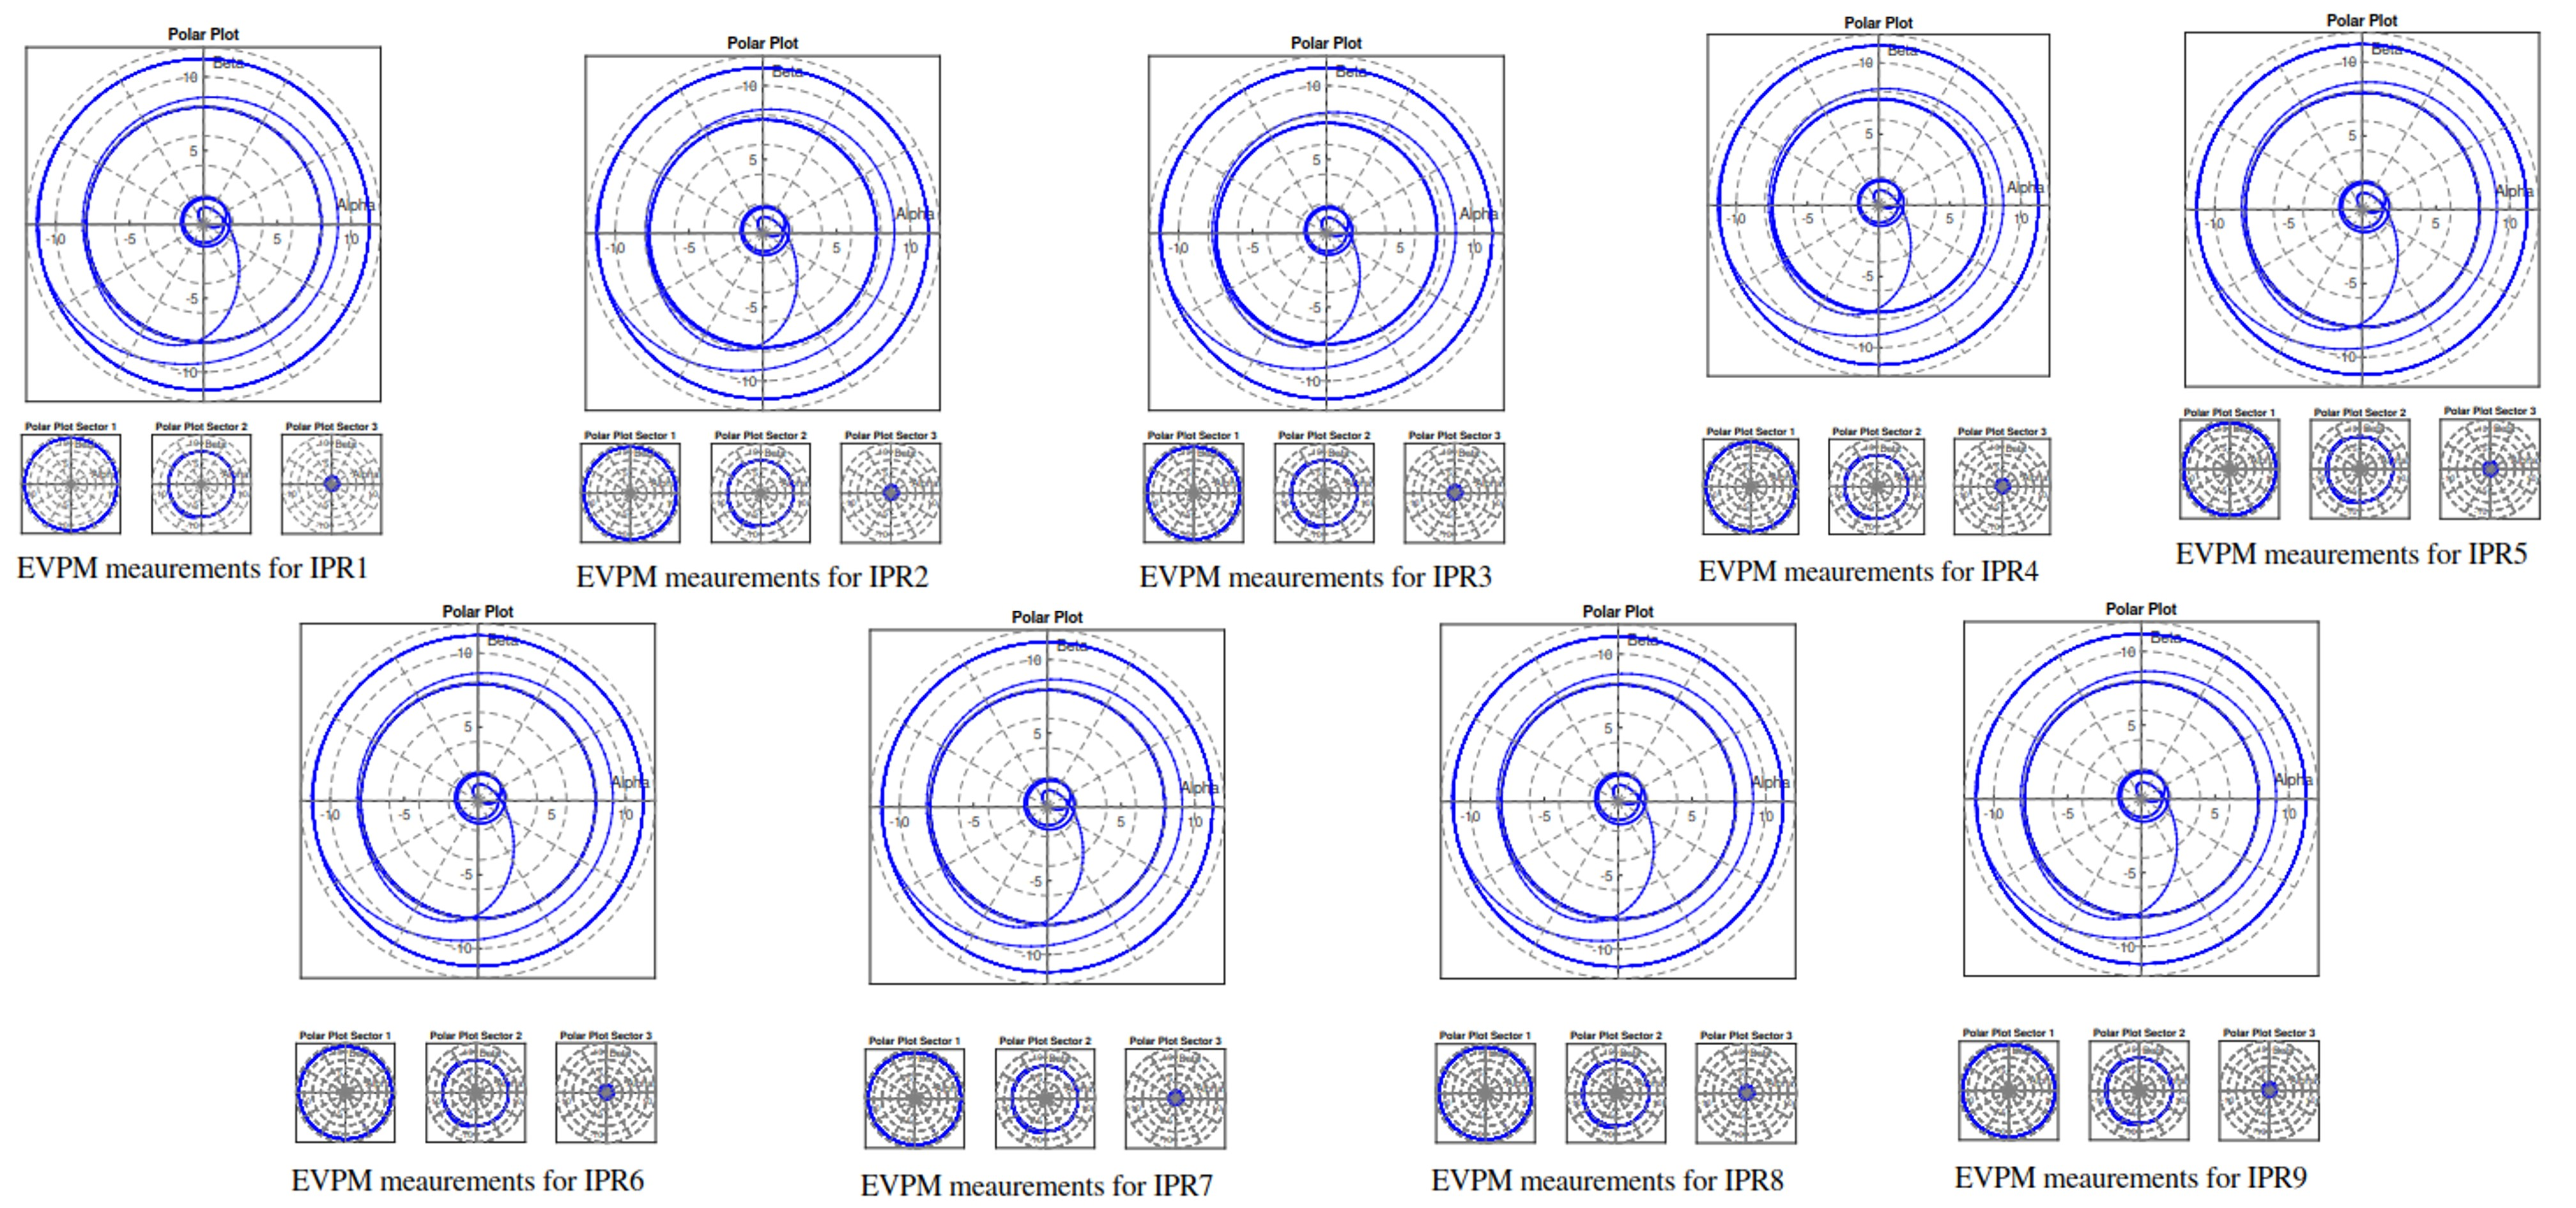
\includegraphics[width=0.95\columnwidth]{images/chapter_5/Ch5F19.jpg}
	\caption{Figure Typical architecture of a Convolutional Neural Networks}
\end{figure}

\section{Summary} 

The research focuses on:\\
	Enhancing the reliability and security of distribution networks with DG integration.\\
	Addressing the challenges posed by DG units, especially during fault conditions.\\
	Leveraging advanced technologies like AI and ML to improve protection performance.\\
	Developing comprehensive protection strategies for microgrids.\\
Proposed Solutions:\\
	Enhanced Voltage Protection Module (EVPM).\\
	Comprehensive Protection Strategy for Microgrids.\\
	AI-Based Enhanced Voltage Protection Module (AI-VPM).\\



